This section consists of the robot arm, where the actual movement of the robot happens along with the application, which would be the paintball marker associated with it. The robot arm receives commands from the Controller, which gives it instructions on how it can move the joints, linear rail, and the pneumatic line for the trigger to shoot the paintball. These communication 


\subsection{Layer Hardware}
There are multiple hardware components for this layer. This layer consists of the joints that are controlled by the program in the computer. There is also pneumatic portion which controls the air that will flow through the solenoid valves. The system is also integrated with a linear rail which will control the linear movement of the entire robot arm. These systems are connected to the robot controller which controls these movements and enable communication with the controller.

\subsection{Layer Operating System}
The robot arm uses MELFA Works Operating System.

\subsection{Layer Software Dependencies}
The software dependencies include the use of RT Toolbox3 software to program the movement of the joints, GX Works software to control the PLC and a USB connection to enable the communication between the robot arm and the controller. 

\subsection{Subsystem 1}
Joints are a hardware component of the robot arm that gives the robot a specific orientation to carry out certain tasks. This will require communication from the robot controller and software, RT Toolbox3, which will give it specific orientation.

\begin{figure}[h!]
	\centering
 	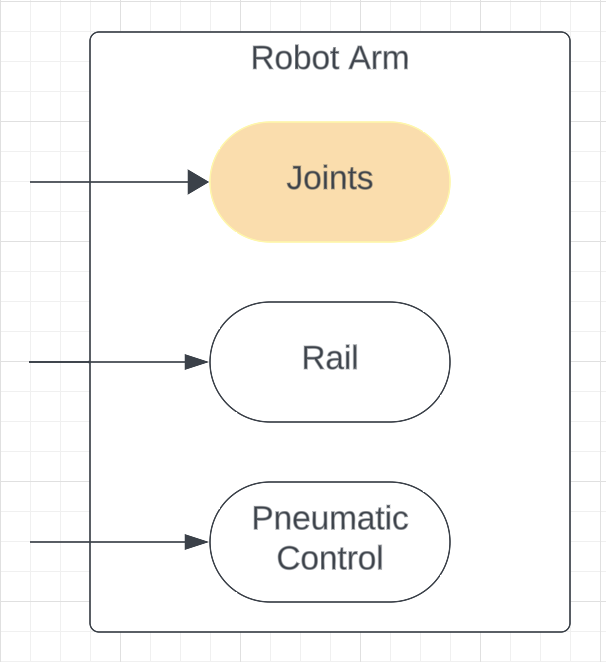
\includegraphics[width=0.60\textwidth]{images/joints.png}
 \caption{Joints Subsystem}
\end{figure}

\subsubsection{Subsystem Hardware}
This subsystem has encoders which communicates the speed of joints back to controller, so that they can adjust. They also have automatic braking system embedded into them to quickly brake if E-stops are enabled. 

\subsubsection{Subsystem Operating System}
Joints use the MELFA Works Operating System to control their orientation and movement.

\subsubsection{Subsystem Software Dependencies}
These joints require the use of RT Toolbox3 for their movement and orientation.

\subsubsection{Subsystem Programming Languages}
The programs of their movement is written in MELFA BASIC VI.

\subsubsection{Subsystem Data Structures}
Some data structures utilized by these joints are joint state and trajectory data structure which give information to the joints on where to move.

\subsubsection{Subsystem Data Processing}
We will be using the joints coordinates given in degrees in order to control their movements. They will be given in a tuple, and we will set boundaries on the limits on where the joints can move.


\subsection{Rail}
Rail is component of the RV8 robot arm which can move all the joints on a linear plane. This gives the robot arm more space to operate and more room in order to perform tasks on a wider plane. The rail receives commands from the servo amplifier which communicates with the robot controller.

\begin{figure}[h!]
	\centering
 	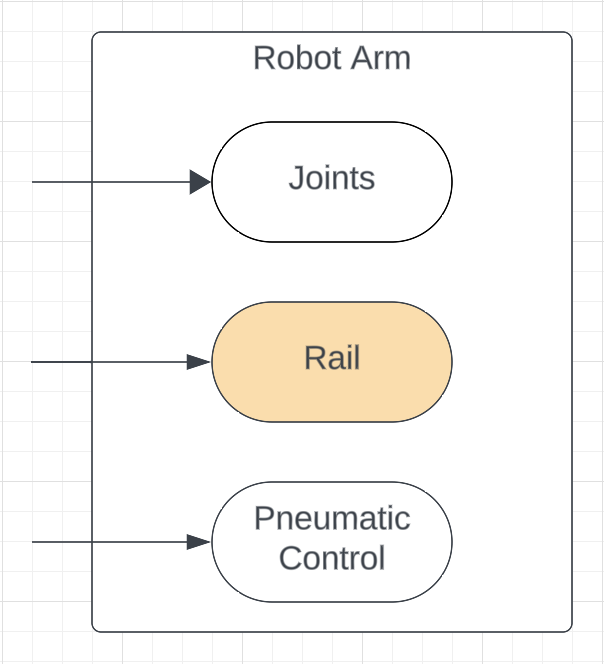
\includegraphics[width=0.60\textwidth]{images/rail.png}
 \caption{Rail Subsystem}
\end{figure}

\subsubsection{Subsystem Hardware}
This subsystem has servo motor which gives the rail its motion. The servo motor communicates with the servo amplifier. The servo motor also consists of encoders which controls the speed of the rail. It also consists of a braking system which limits it from movement when the robot arm is powered off.

\subsubsection{Subsystem Operating System}
Linear rail use the MELFA Works Operating System to control their movement.

\subsubsection{Subsystem Software Dependencies}
The rail requires RT Toolbox3 to program its movements.

\subsubsection{Subsystem Programming Languages}
The programs of their movement is written in MELFA BASIC VI.

\subsubsection{Subsystem Data Structures}
Data structures utilized by these consist of movement data structures, especially those of kinetic and dynamic structures, position, which help enable the movement of the linear rail.

\subsubsection{Subsystem Data Processing}
For data processing, the linear rail will use have a set origin, and can be configured according to the application. This will include adjusting its movement according the image that will be processed.




\subsection{Pneumatic Control}
Pneumatic system is connected to the RV8 robot and controls the air pressure that will travel through the robot. The wiring is connected to the PLC which, through the programs, will control the air pressure that will travel through the pipes. The pneumatic control will be connected through solenoid valves which will control the compressed air.

\begin{figure}[h!]
	\centering
 	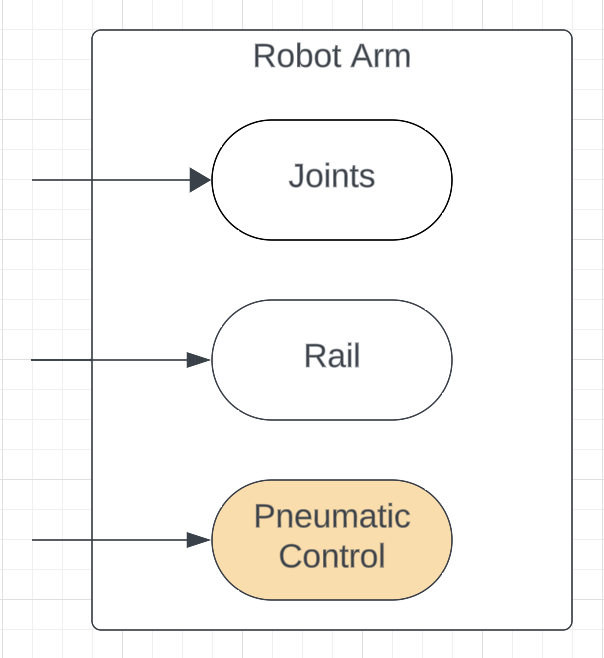
\includegraphics[width=0.60\textwidth]{images/pneumatic.png}
 \caption{Pneumatic Control Subsystem}
\end{figure}

\subsubsection{Subsystem Hardware}
This subsystem has PLC which will be programmed in order to control the compressed air, and has solenoid valves will be connected to the PLC. This will help the compressed air to trigger the paintball marker.

\subsubsection{Subsystem Operating System}
Pneumatic Control use the MELFA Works Operating System to control their movement.

\subsubsection{Subsystem Software Dependencies}
The pneumatic control requires GXWorks3 for programming

\subsubsection{Subsystem Programming Languages}
The programs of their movement is written in Ladder Logic.

\subsubsection{Subsystem Data Structures}
Data structures utilized by these consist of valve state data structures, which also consists pressure and flow data structures. These will be used in order to control the compressed air flow.

\subsubsection{Subsystem Data Processing}
For data processing, the pneumatic control will use to activate and deactivate solenoid valves. There are also going to be sensors that will transmit data regarding the proper functioning of the solenoid valves.